%%%%%%%%%%%%%%%%%%%%%%%%%%%%%%%%%%%%%%%%%%%%%
%%                 PŘÍLOHY                 %%
%%%%%%%%%%%%%%%%%%%%%%%%%%%%%%%%%%%%%%%%%%%%%
\chapter{Přílohy}
\label{prilohy}
\section{Diagram sestavení geometrie hranic}
\begin{figure}[H]
	 \centering
      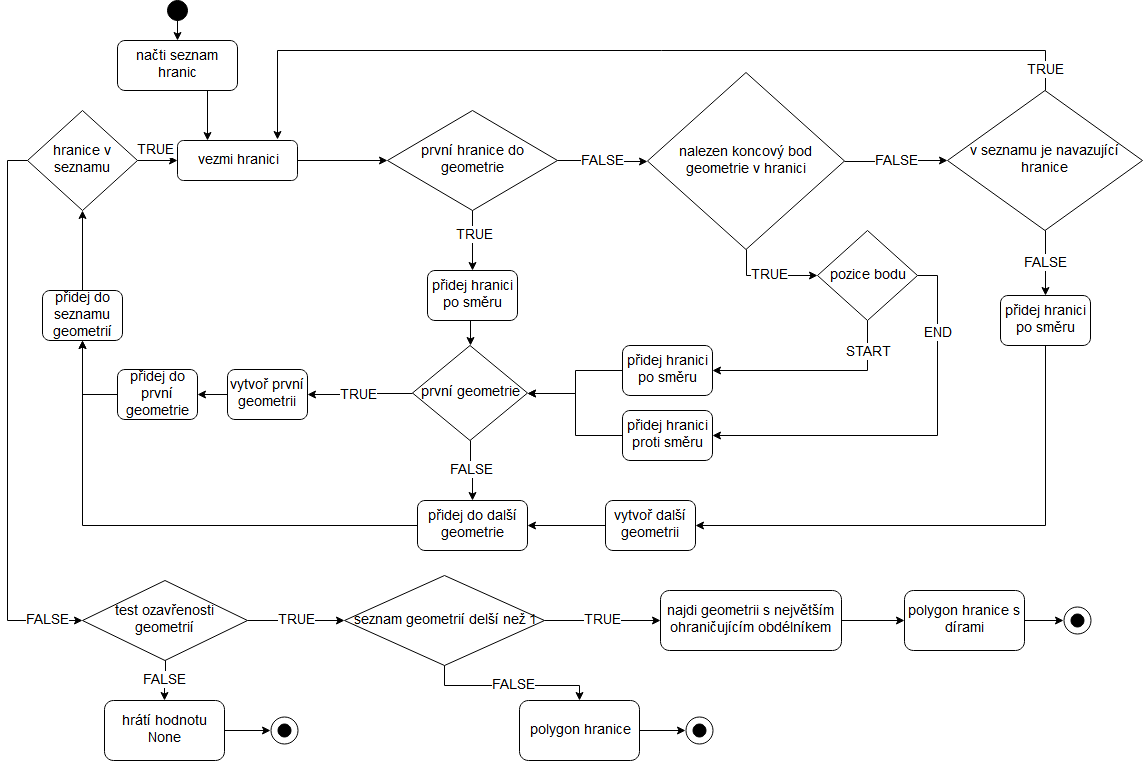
\includegraphics[width=15cm]{./pictures/Diagram_sestaveni_geometrie_hranic.png}
      \caption{zdroj:vlastní}
      \label{fig:logika_geometrie}
  \end{figure}
  
 \section{Ukázka načtení dat pomocí zásuvného modulu v prostředí QGIS}
 \begin{enumerate}
 \item{Spuštění zásuvného modulu kliknutím na ikonu \texttt{Otevřít prohlížeč VFK}}
  \begin{figure}[H]
	 \centering
      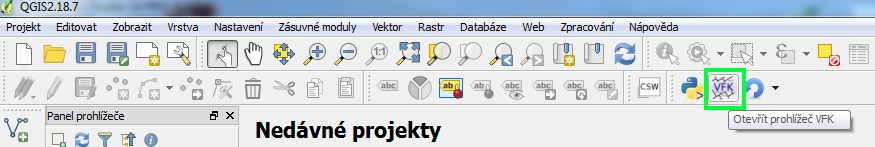
\includegraphics[width=15cm]{./pictures/nacteni_1kr.png}
      \caption{Ikona zásuvného modulu(označena zeleně)}
      \label{fig:1kr_nacteni}
  \end{figure}
  
  \item{Pro výběr VFK souboru stiskněte tlačítko \texttt{Procházet}(označeno zeleně)}
  \begin{figure}[H]
	 \centering
      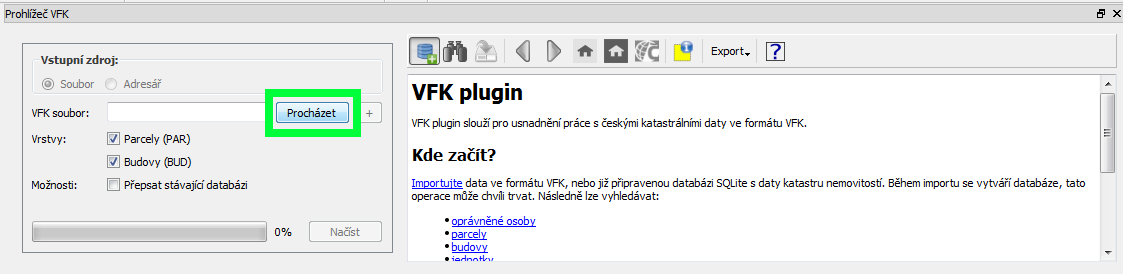
\includegraphics[width=15cm]{./pictures/nacteni_2kr.png}
      \caption{Výběr VFK souboru}
      \label{fig:2kr_nacteni}
  \end{figure}
  
  \item{Zvolení VFK souboru a výběr kliknutím na tlačítko \texttt{Otevřít}, výběr možný i dvojklikem}
  \begin{figure}[H]
	 \centering
      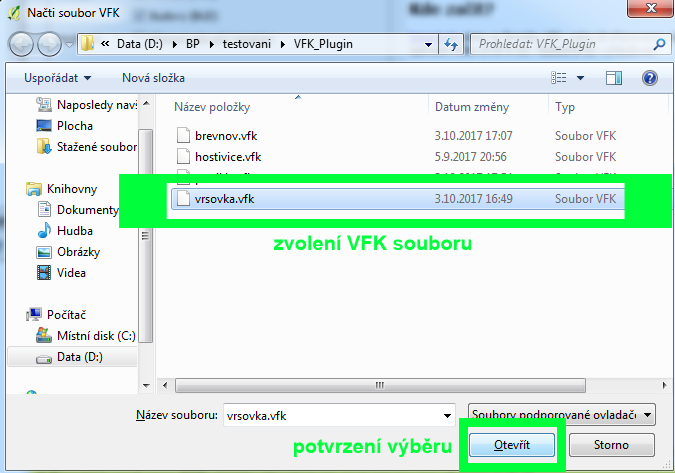
\includegraphics[width=15cm]{./pictures/nacteni_3kr.png}
      \caption{Načti soubor VFK}
      \label{fig:3kr_nacteni}
  \end{figure}
  
  \item{Kliknutím na tlačítko \texttt{Načíst} se spustí načítání dat}
  \begin{figure}[H]
	 \centering
      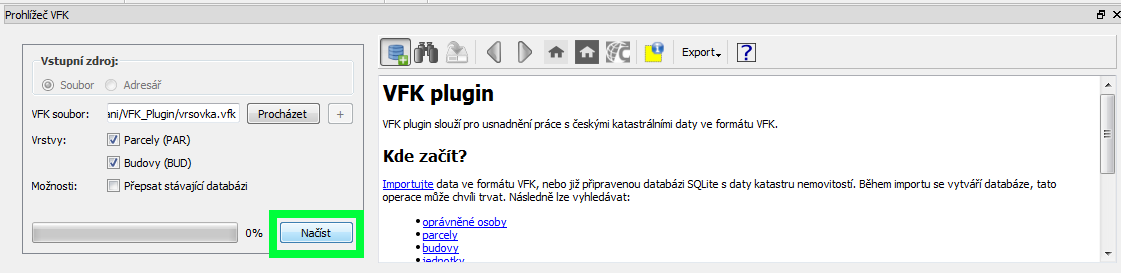
\includegraphics[width=15cm]{./pictures/nacteni_4kr.png}
      \caption{Spuštění načítání}
      \label{fig:4kr_nacteni}
  \end{figure}
  
  \item{Probíhá načítání}
  \begin{figure}[H]
	 \centering
      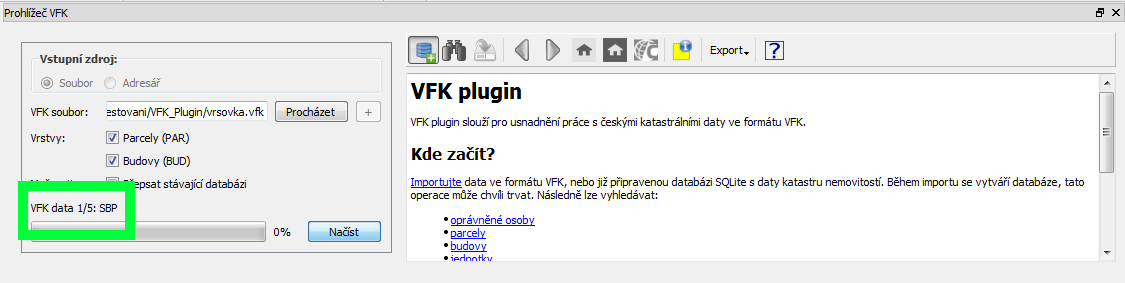
\includegraphics[width=15cm]{./pictures/nacteni_5kr.png}
      \caption{Načítání v procesu, může chvíli trvat}
      \label{fig:5kr_nacteni}
  \end{figure}
  
   \item{Data se po načtení sama zobrazí}
  \begin{figure}[H]
	 \centering
      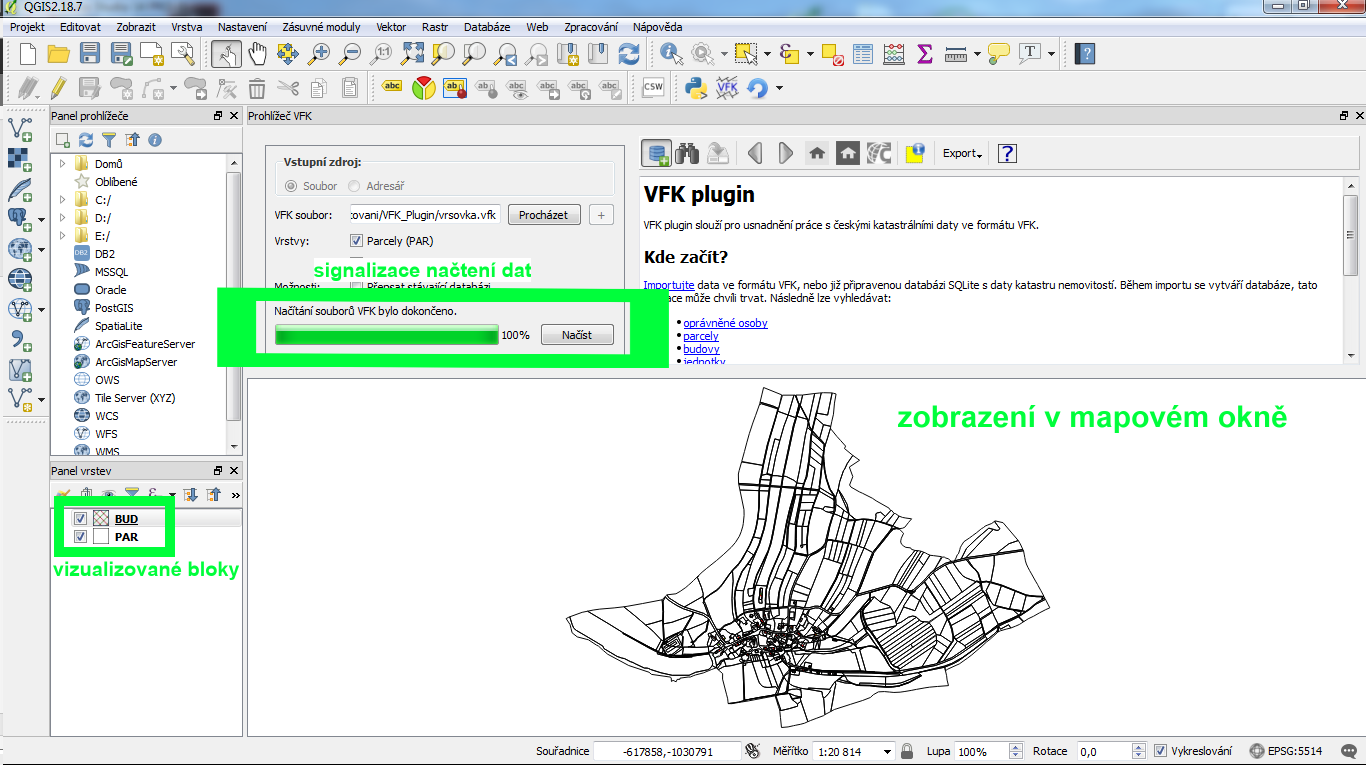
\includegraphics[width=15cm]{./pictures/nacteni_6kr.png}
      \caption{Načtená data pro obec Vršovka}
      \label{fig:6kr_nacteni}
  \end{figure}
 \end{enumerate}
 
 \section{Obsah CD}